\chapter{Conclusions} \label{chap:conc}

Over the last five chapters, we have introduced two new machine-learning frameworks, applied them to various surveys, and used these to draw new insights into galaxy formation and evolution. In this chapter, we will provide a brief summary of the key takeaways from this work and also provide the reader with an outlook for the future.

\section{Publicly Available Algorithms \& Data Products} \label{sec_conc:public_products}

The open-source movement began in the early years of the new millennium and has revolutionized how we develop, distribute, and interact with computing and software. Making source code freely available fosters a collaborative environment where knowledge is shared, and innovation is encouraged. This has had a significant impact on computing within astronomy as well --- over time, more astronomers (although not all) have chosen to make their catalogs, analysis pipelines, and software source code freely available. 

As strong believers in the open source movement, we have released the entirety of the source code, trained machine learning models, and catalogs that were developed and used as a part of this thesis. We have also created extensive documentation and tutorials for all our ML frameworks to enable other astronomers to use these frameworks easily. Below we provide a summary of the various data-products

\begin{enumerate}
    \setlength\itemsep{-0.1em}
    \item \gamornet{} Data Products
    \begin{itemize}
    \setlength\itemsep{-0.1em}
        \item \href{https://github.com/aritraghsh09/GaMorNet}{Source Code}
        \item \href{https://gamornet.readthedocs.io/en/latest/}{Documentation}
        \item \href{https://gamornet.readthedocs.io/en/latest/tutorials.html}{Tutorials}
        \item \href{https://gamornet.readthedocs.io/en/latest/usage_guide.html#trained-models}{Trained Model for SDSS $z\sim0$ data}
        \item \href{https://gamornet.readthedocs.io/en/latest/usage_guide.html#trained-models}{Trained Model for CANDELS $z\sim1$ data}
    \end{itemize}
    \item \gampen{} Data Products
        \begin{itemize}
        \setlength\itemsep{-0.1em}
            \item \href{https://github.com/aritraghsh09/GaMPEN}{Source Code}
            \item \href{https://gampen.readthedocs.io/en/latest/index.html}{Documentation}
            \item \href{https://gampen.readthedocs.io/en/latest/Tutorials.html}{Tutorials}
            \item \href{https://gampen.readthedocs.io/en/latest/Public_data.html}{Trained Model for HSC $z < 0.75$ data}
            \item \href{https://colab.research.google.com/github/aritraghsh09/GaMPEN/blob/master/tutorials/Autocropping.ipynb}{Standalone Auto-cropping Module}
        \end{itemize}
    \item Catalogs
    \begin{itemize}
    \setlength\itemsep{-0.1em}
        \item \href{https://gamornet.readthedocs.io/en/latest/usage_guide.html#prediction-tables}{Morphological Catalog of $\sim100,000$ SDSS $z\sim0$ galaxies}
        \item \href{https://gamornet.readthedocs.io/en/latest/usage_guide.html#prediction-tables}{Morphological Catalog of $\sim20,000$ CANDELS $z\sim1$ galaxies}
        \item \href{https://gampen.readthedocs.io/en/latest/Public_data.html#prediction-tables}{Structural Parameters \& Associated Uncertainties for $\sim8$ million $z <0.75$ HSC galaxies}
    \end{itemize}
\end{enumerate}

We believe that the above-mentioned data products will be extremely beneficial to the wider astronomical community. Both \gamornet{} and \gampen{} are extremely well suited to perform morphology determination in upcoming large surveys such as Rubin-LSST, NGRST, Euclid, and the extensive amount of archival imaging data available to astronomers. The trained models we have released will be beneficial for performing morphology determination in the specific surveys they were trained for, and these ML models can also be the starting point for fine-tuning for other surveys. Finally, our catalogs will serve as an important resource for studying galaxy formation and evolution --- especially our HSC  catalog, the only one of its kind and one of the largest structural parameter catalogs currently available in astronomy. 

\section{Key Breakthroughs \& Takeaways} \label{sec_conc:takeaways}

In this section, we summarize the key breakthroughs and takeaways from Chapters \ref{ch:gamornet} - \ref{chap:morph_den}

\subsection{Technical Breakthroughs} \label{sec_conc:tech_breakthroughts}
This thesis has conclusively demonstrated the effectiveness of ML frameworks in performing morphology determination on both ground and space-based imaging data sets. It has solved a host of key challenges that will enable ML fireworks to be applied at scale to the large imaging data sets of the next decade, such as Rubin-LSST, NGRST, and Euclid. 

\subsubsection{Quick \& Accurate Morphology Determination Across the Board } 
In Chapters \ref{ch:gamornet} - \ref{chap:hsc_morph}, we conclusively demonstrated that our novel ML frameworks can be effectively applied to galaxies at different epochs of cosmic time with data sets of varying resolution, pixel-scale, and signal-to-noise ratio. They can determine broad morphological classifications (such as disk-dominated, bulge-dominated, etc.) and accurate determinations of structural parameters (such as radius, bulge-to-total light ratio, etc.). \gamornet{} achieved an overall accuracy  of $\gtrsim 95\%$ on SDSS $z\sim0$ and CANDELS $z\sim1$ galaxies; while \gampen{}'s predicted posterior distributions were shown to be extremely well calibrated with $\lesssim 5\%$ deviation. These results conclusively establish that ML morphology determination frameworks (of the same structure) can be universally applied to data of varying quality at different epochs of time and achieve excellent results.

In Chapter \ref{chap:hsc_morph}, we put our ML frameworks head-to-head with light profile fitting frameworks using simulated data. We demonstrated that \gampen{}'s determination of structural parameters is better than that of light-profile-fitting tools, especially for smaller and fainter galaxies. In Chapters \ref{ch:gamornet} - \ref{chap:hsc_morph}, we also demonstrated that ML frameworks can move beyond single-component \sersic{} profiles and perform multi-component analysis like bulge + disk decomposition accurately. This result will serve as an important first step for more such careful comparisons and make ML frameworks like \gampen{} the method of choice for structural parameter determination in large data sets.

 
Although often taken for granted, it is helpful to state the speed at which our frameworks can determine morphology. It takes $\sim12-16$ hours to train our ML frameworks on two state-of-the-art NVIDIA\footnote{\href{https://www.nvidia.com/en-us/}{https://www.nvidia.com/en-us/}} GPUs. Once trained it takes our frameworks $<10^{-3}$ seconds to perform one sampling of structural parameters for a single galaxy. Therefore, to predict full posterior distributions of structural parameters for a sample of $\sim1$ million galaxies on simply two GPUs, it takes $<5$ days. Of course, this speeds up linearly if one uses more GPUs. Therefore, our ML frameworks are completely ready for the billion galaxy samples expected from upcoming surveys.


\subsubsection{Successful Training Without Needing Large Real Data-sets}
We put forward in Chapters \ref{ch:gamornet} \& \ref{chap:hsc_morph} a novel technique to perform morphology determination without needing large pre-classified data sets. We showed that by first training our frameworks on semi-realistic simulations of galaxies (which are computationally cheap to make); and then fine-tuning the trained frameworks using a small amount of real data, we can achieve at-par or better accuracies than light profile fitting methods. This two-step method ensures that:- a) the base network has been trained using simulation data where we have access to the robust ground-truth morphological parameters; b) we need a very small amount of real data for training. Following this method, we produced the first large structural parameter catalog for HSC data while using $<1\%$ of the total dataset for training. This provides a viable pathway for how structural parameter determination can be performed in upcoming large surveys.  

\subsubsection{Prediction of Robust Uncertainties}
In Chapter \ref{ch:gampen}, we demonstrated how we can incorporate the full covariance matrix into our loss function and combine that with the Monte Carlo Dropout technique to incorporate both epistemic and aleatoric uncertainties into our predictions. This enabled us to predict extremely well-calibrated and accurate posterior distributions for all the structural parameters --- the overall deviation from theoretical values were shown to be $\lesssim 5\%$. This represents a major breakthrough --- no previous ML morphology frameworks could determine uncertainties. We also demonstrated that our predicted uncertainties represent a significant improvement over approximate estimates of errors obtained from traditional morphological analysis tools like GALFIT, Galapagos, or ProFit -- which underestimate the true uncertainties by $\sim15-60\%$ depending on the flux of the galaxy being analyzed. 


\subsubsection{Automated Data Pre-Processing} 
We had outlined previously in \S \ref{sec_intro:challenges} how one of the challenges with ML frameworks is the requirement to use cutouts of a fixed size. Therefore, astronomers have often resorted to using large cutout sizes --- which often results in typical cutouts containing other galaxies in the frame, often leading to misclassifications and less accurate results. We have presented a potential solution to this challenge in Chapters \ref{ch:gampen} \& \ref{chap:hsc_morph} --- by using a Spatial Transformer Network, we can automatically crop galaxies to an optimal size before determining their morphology. The STN is integrated within \gampen{} and does not need any additional training. We have demonstrated that this enables us to apply \gampen{} to galaxies across a wide range of redshifts, sizes, and brightness. We have made the STN also available as a standalone framework (see \S \ref{sec_conc:public_products}). This will enable users to crop a large number of cutouts to an optimal size (when radius measurements are not available beforehand) in preparation for any analysis of their choice.  

\subsection{Science Takeaways} \label{sec_conc:science_takeaways}
As outlined in \S \ref{sec_conc:tech_breakthroughts}, we made some key technical breakthroughs in this thesis --- let us now summarize the early science that these breakthroughs have already enabled. 

\subsubsection{Galaxies In Denser Environments Are Larger} \label{sec_conc:morph_den} 

Although it has been known since the late 1900s that galaxy morphology is strongly correlated with local environment, the question of whether galaxy sizes are correlated with environment has not been well-established at all. As summarized in Chapter \ref{chap:morph_den}, different studies have reported positive, negative or no correlation, typically using samples of $\om(10^{2-3})$ galaxies. These conflicting results have primarily been driven by small sample sizes, the inability to account for the proper level of uncertainty in radius measurements, and the lack of uniformity in samples used within the same study. Our ML frameworks, with their ability to process large volumes of data and predict robust uncertainties put us in a unique position to tackle this problem for the first time. 

We used the structural parameters determined by \gampen{} using the excellent imaging quality of HSC to perform the first comprehensive study of the variation of galaxy radius with large-scale structure beyond $z > 0.2$. We used a sample of $\sim3$ million HSC galaxies in the redshift range $0.3 \leq z < 0.7$ with masses down to $\log M/M_{\odot}\sim8.5$. We studied the variation of both radius as well as morphology on a 10 comoving Mpc scale -- thus focusing on the large-scale environmental effect by taking advantage of the wide-field coverage of Hyper Suprime-Cam ($\sim 360$ deg$^2$). Our large sample size (at least $100\times$ compared to past studies) allows us to robustly confirm/reject the presence of correlations with high statistical significance. 

We confirmed with $>5\sigma$ confidence that galaxy radius is indeed correlated with environment. At the scales considered, galaxies in denser environments are larger than galaxies of similar mass in less dense environments. We found the nature of the correlation to be dependent on redshift and a weak function of mass and galaxy morphology. We found the correlation to be strongest at $z < 0.5$ and become weaker/disappear at $z \geq 0.5$. We found the overall correlation at lower redshifts to be persistent across all sub-samples we study -- disk-dominated, bulge-dominated, star-forming, quiescent galaxies. We also found the correlation to be marginally stronger at higher stellar masses. 

We posit that the above variations are a result of how dark-matter halos collapse and how structure formation takes place in halos. Due to assembly bias, larger dark matter halos (of the same mass) typically reside in denser environments, and  halos (of the same mass) with higher concentration and spin cluster more strongly. Many galaxy formation models have predicted that the radial sizes of galaxies depend on the spin of their dark matter halos and that galaxy sizes should be proportional to the spin and size of the dark matter halo. Therefore, our observed correlations seem to provide preliminary evidence that these theoretical models might be correct --- although detailed one-to-one comparison simulation studies are needed to confirm the exact cause for the observed correlations.

At $z > 0.5$, although the overall correlation is much weaker, we can observe a stronger correlation for bulge-dominated and quiescent systems compared to disk-dominated and star-forming galaxies. This correlation gets even stronger for galaxies beyond a critical stellar mass of $\log M/M_{\odot} \sim 11.25$. We posit that these correlations result from how structural growth occurs in bulge-dominated/quiescent systems. Minor, dry mergers dominate size growth in these systems, especially at higher masses. Given that mergers are more efficient and frequent in denser environments, bulge-dominated/quiescent systems in dense environments undergo a more rapid size evolution compared to their equally massive counterparts in lower-density environments. The increased correlation for bulge-dominated/quiescent systems is mostly observed in the higher redshift bins --- this could be because mergers are thought to be more prevalent at higher redshifts. Since size growth at lower masses and for disk-dominated/star-forming systems are not dominated by mergers, it is not surprising that our observed correlation is weaker/absent for these cases. 

\subsubsection{Morphology is An Effective Tool to Isolate Galaxies on Different Evolutionary Pathways} \label{sec_conc:color_mass}

In Chapter \ref{ch:gamornet}, we used \gamornet{} derived morphologies to study the quenching of star formation in  $z\sim0$ (SDSS) and $z\sim1$ (CANDELS) galaxies by examining their color-mass diagrams. For both the samples, we found that both bulge- and disk-dominated galaxies span the entire range of colors (i.e., we see examples of red disk-dominated galaxies and blue bulge-dominated galaxies). As expected, the disk-dominated galaxies peak in the blue cloud, while the bulge-dominated galaxies dominate the red sequence. The green valley is not a feature for either morphology; that is, there is no bimodality. Rather, the number density of galaxies declines monotonically from a red or blue peak. Thus, the green valley only arises when plotting the color-mass diagram of all galaxies together, as was first pointed out for $z\sim0$ galaxies by using Galaxy Zoo morphologies. 

The disk-dominated galaxies peak in the blue cloud and then gradually extend to the red sequence, suggesting that quenching in disks is a secular process. Conversely, bulge-dominated galaxies in both samples peak  in  the  red  sequence,  with  very few precursors in the green valley and blue cloud. This is consistent with a scenario in which bulge-dominated galaxies form from major mergers of disk-dominated blue galaxies and then are rapidly quenched through the green valley. Our results are largely consistent with previous studies of star formation and morphology.

Finally, our large sample sizes compared to previous studies allowed us to put better constraints on the fractions of rare objects. We could constrain the population of red disks found at high masses to be at $\sim14$\% of disks at $z\sim0$ and 2\% of disks at $z \sim 1$. These fractions indicate that although disks undergo a gradual decline in star formation as opposed to being rapidly quenched through the green valley into the red sequence; at high masses, there are relatively more red disk-dominated galaxies; and this fraction is higher for nearby galaxies compared to higher redshifts. This suggests that higher halo masses may play a role in shutting off the gas supply and quenching star formation. 

\begin{wrapfigure}{R}{0.45\textwidth}
\centering
\vspace{-0.3in}
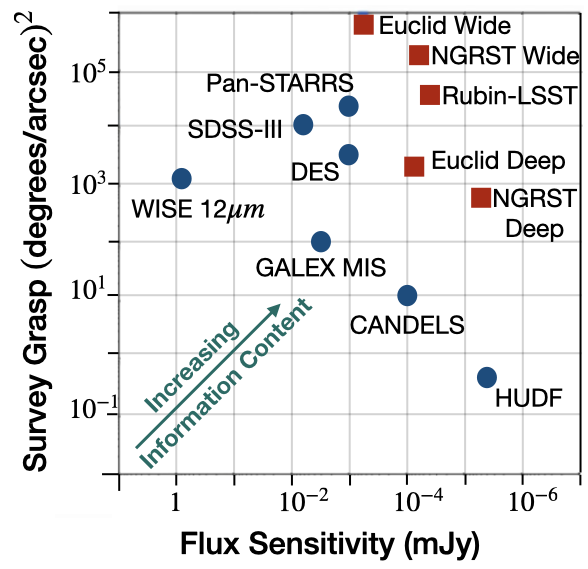
\includegraphics[width=0.45\textwidth]{surveys.png}
\vspace{-0.3in}
\caption{ The next decade in astronomy will witness some of the most information-rich surveys (red squares) when compared to existing data (blue circles), some of which we have used in this work}
\label{fig:surveys}
\vspace{-0.2in}
\end{wrapfigure}


\section{Final Thoughts \& Looking Ahead} \label{sec_conc:future}
As we have demonstrated in this thesis, careful model development and extensive testing form the basis of being able to use machine learning effectively in astronomy. In this work, we were able to build and introduce new innovative ML frameworks, test them extensively, and finally, use them to extract new insights into galaxy formation and evolution.

However, this is just the ``tip of the iceberg". As Fig. \ref{fig:surveys} shows, we will witness some of the most information-rich galaxy surveys over the next decade. Rubin-LSST will probe an area similar to Pan-STARRS ($\sim~20,000$ deg$^2$), but $\sim4$ magnitudes deeper and up to $z\sim5$; providing photometry for $\sim10$ billion galaxies. NGRST, with a field-of-view 100 times that of Hubble, will perform a high-latitude survey that will cover $\sim2000$ deg$^2$ with a sensitivity of $m\sim28$, yielding $\sim1$ million galaxies. Euclid will perform imaging at similar bands but with a mirror half the size of NGRST. It will perform a wide-field survey over $\sim15,000$ deg$^2$ down to $m\sim24.5$. Besides the wide field surveys, NGRST and Euclid’s combined deep fields will allow us to probe the same flux sensitivity of the Hubble Ultra Deep Field, but over a $\sim10^3$ larger area 

Rubin-LSST, Euclid, and NGRST together represent a once-in-a-generation opportunity that will transform our knowledge and understanding of the universe. However, to harness the full potential of these datasets, a paradigm shift is necessary for the tools we have used over the decades to study different physical properties of galaxies. The tools and methods developed in this thesis represent an important step in this direction --- astronomers will use/fine-tune our methods and models to apply them to these new datasets. 

 The last two decades of research in extragalactic astronomy have shown that it is possible to construct a self-consistent model of galaxy evolution based on the paradigm that galaxies form hierarchically around peaks in the dark matter density distribution. However, we have a long way to go before declaring victory in our understanding of galaxy evolution. Many of these unsolved challenges are driven by the fact that the process of galaxy evolution is stochastic in nature. The hierarchical paradigm tells us statistically when dark matter peaks of various masses and overdensities collapse and virialize, on top of which we layer our understanding of gas cooling, star formation, and feedback. Because the overall process is stochastic, some of the most important tests of the models must be performed against large statistical data sets. These data sets must be uniform, with known, well-defined selection functions. As demonstrated in this thesis, when such large datasets are combing with appropriate novel algorithms, one can derive new insights into how galaxies form and evolve. Based on this, one might indeed say that the future looks bright and hopeful --- the next generation of large surveys and powerful computational algorithms will herald a new age of discovery in astronomy. 


